% !Mode:: "TeX:UTF-8:Main"
\documentclass{beamer}

\usepackage{tikz}
\usepackage{tikzlings-koalas}
\usepackage{fontspec}
\usetikzlibrary{shapes}
\newfontfamily\notoemoji{Noto Color Emoji}[Renderer=HarfBuzz]

\setbeamertemplate{background canvas}{
  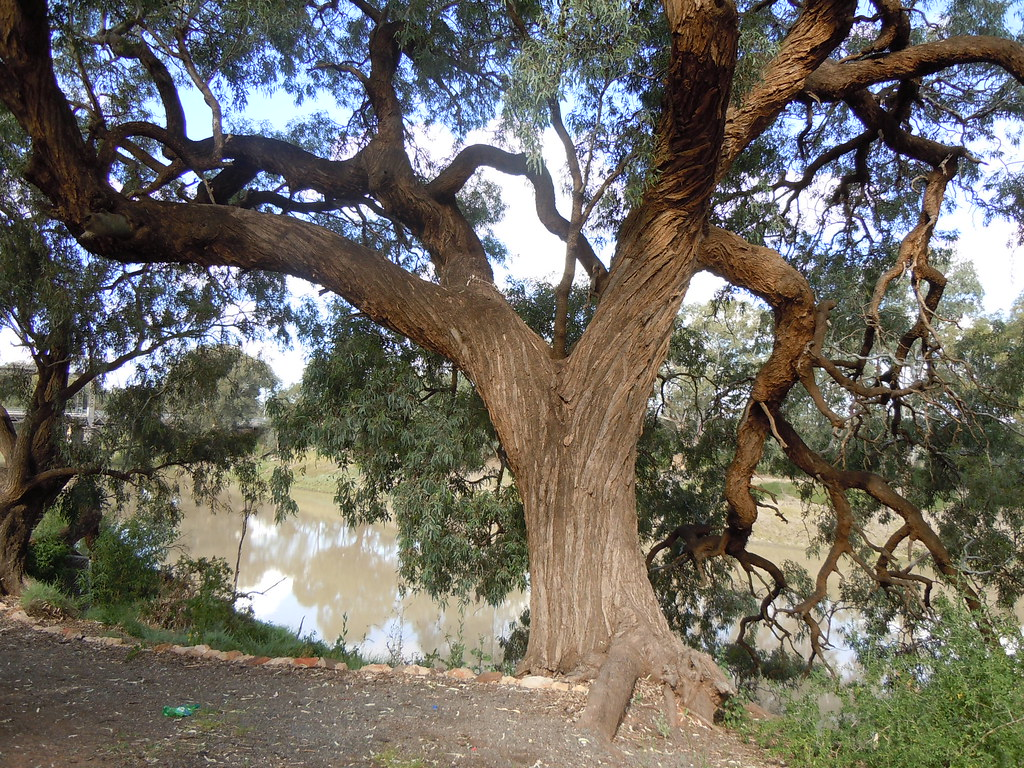
\includegraphics[height=\paperheight]{eukalyptus}
}
\setbeamertemplate{navigation symbols}{}

\begin{document}
\makeatletter\def\thing@strawhat{brown}

\begin{frame}

\vspace*{5.5cm}

\mbox{}\hfill 
  \begin{tikzpicture}[scale=1.5,transform shape]  
  \koala[shift={(0,0.3)}]
  \begin{scope}[overlay]
  \begin{scope}[xshift=-18,rotate=12,yshift=-1.1,scale=1.2]
  \fill[\thing@strawhat,rotate=-15] (0.44,2.0) ellipse[x radius=0.75, y radius=0.1];
  \fill[\thing@strawhat,rotate=-15] (0.1,2.05) rectangle (0.78,2.5);
  \fill[\thing@strawhat,rotate=-15] (0.44,2.5) ellipse[x radius=0.34, y radius=0.08];
  \fill[\thing@strawhat,rotate=-15] (-0.3,2.02) -- (1.18,2.02) -- (0.78,2.2) -- (0.1,2.2) -- cycle;
  \fill[brown!50!black,rotate=-15] (0.44,2.2) ellipse[x radius=0.34, y radius=0.08];
  \fill[brown!50!black,rotate=-15] (0.1,2.2) rectangle (0.78,2.3);
  \fill[\thing@strawhat,rotate=-15] (0.44,2.3) ellipse[x radius=0.34, y radius=0.08];
  \draw[red,rotate=-15] (0.44,2.0) ellipse[x radius=0.75, y radius=0.1];
  
  \node at (1,2.2){\tiny\notoemoji🦘};
  \end{scope}
  \end{scope}
  \end{tikzpicture}\hspace*{3cm}
  	
\end{frame}	

\end{document} 


